
\section{Section 3: Structured Modeling }

\begin{frame}{Training Seq2Seq}
  Seq2Seq is trained to predict the next word \textit{given the true history.}

  \begin{center}
  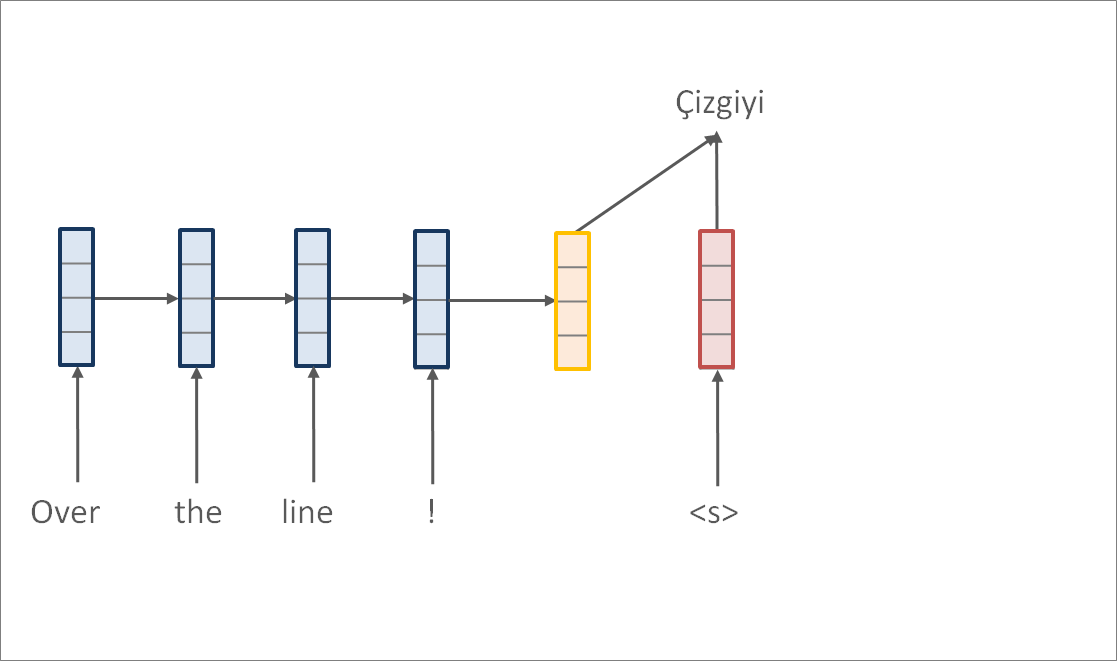
\includegraphics[height=3.5cm, trim={12cm 3cm 7cm 0.5cm}, clip]{nmt-noattn-4}
  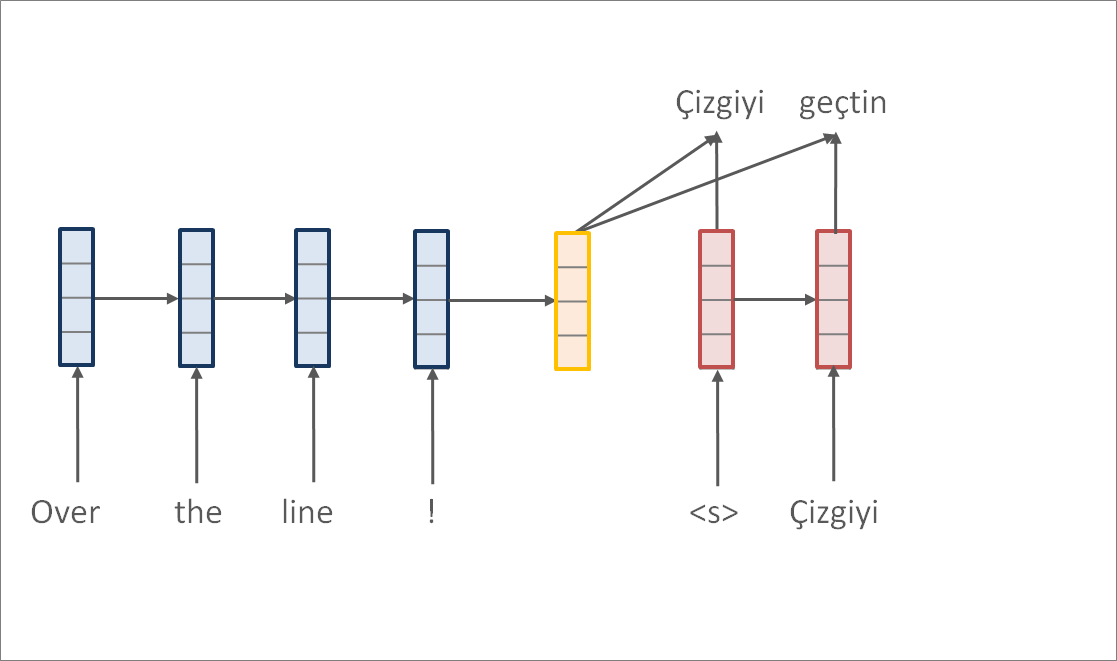
\includegraphics[height=3.5cm, trim={12cm 3cm 3cm 0.5cm}, clip]{nmt-noattn-6}
  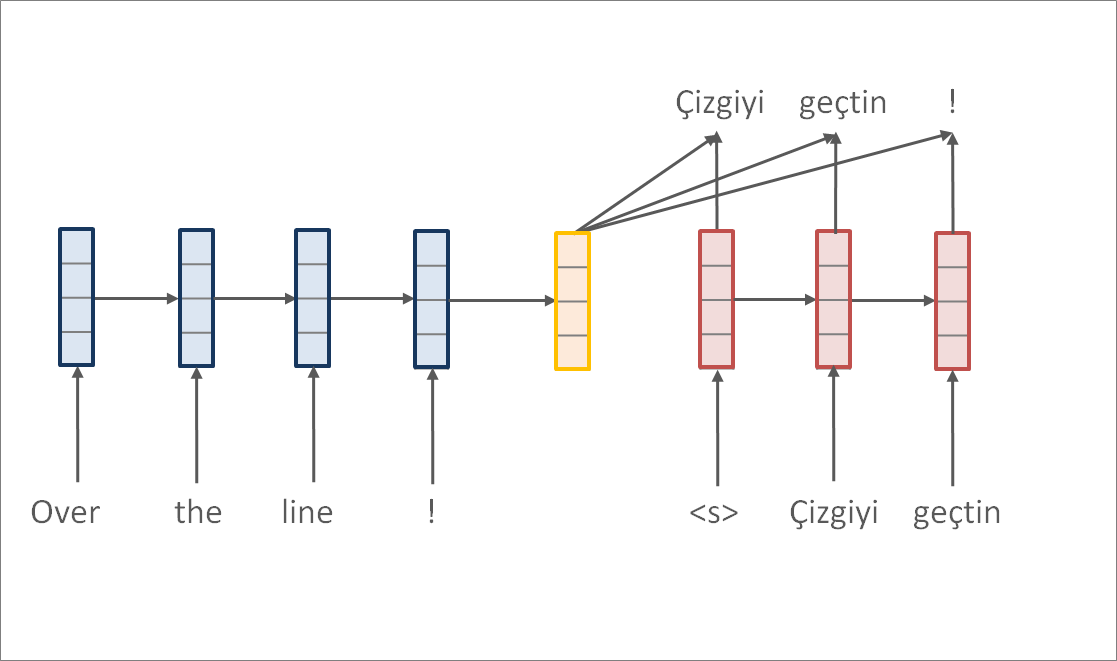
\includegraphics[height=3.5cm, trim={12cm 3cm 0.5cm 0.5cm}, clip]{nmt-noattn-7}
  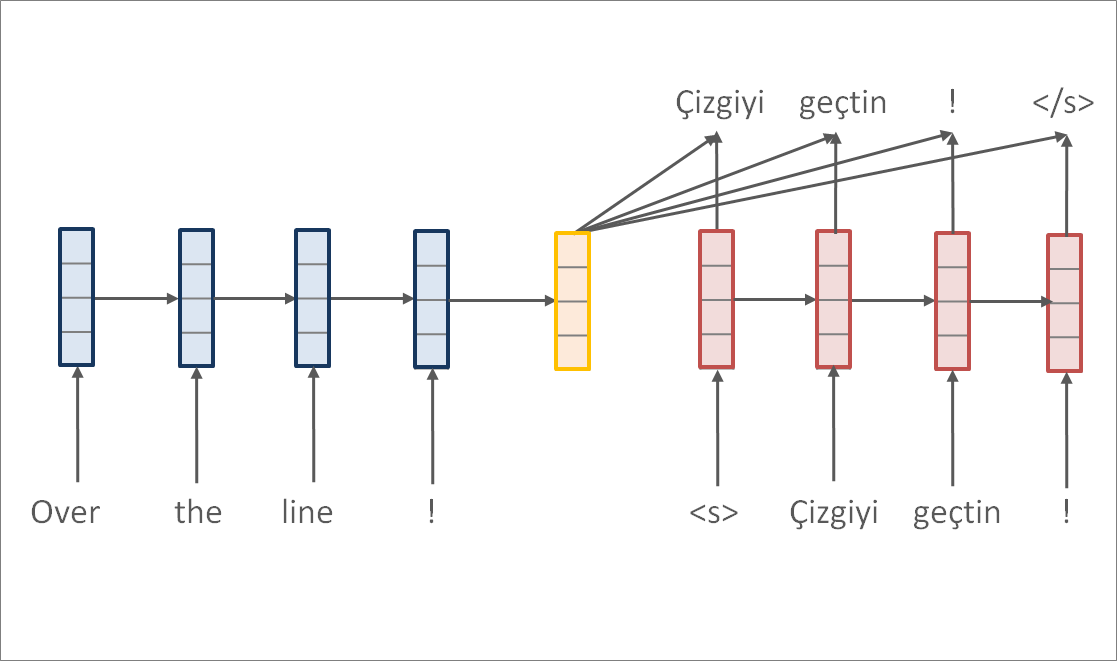
\includegraphics[height=3.5cm, trim={12cm 3cm 0.5cm 0.5cm}, clip]{nmt-noattn-8}
  \end{center}
  Multiclass Classification:
  \[ \text{NLL}(\theta) = -\sum_{t} \log p(y_t |  y_{1:t-1}, \cvec; \theta) \] 
\end{frame}

\begin{frame}{Deploying Seq2Seq}
  Seq2Seq is deployed to predict a next word \textit{given its predictions}.


  \begin{center}
  % 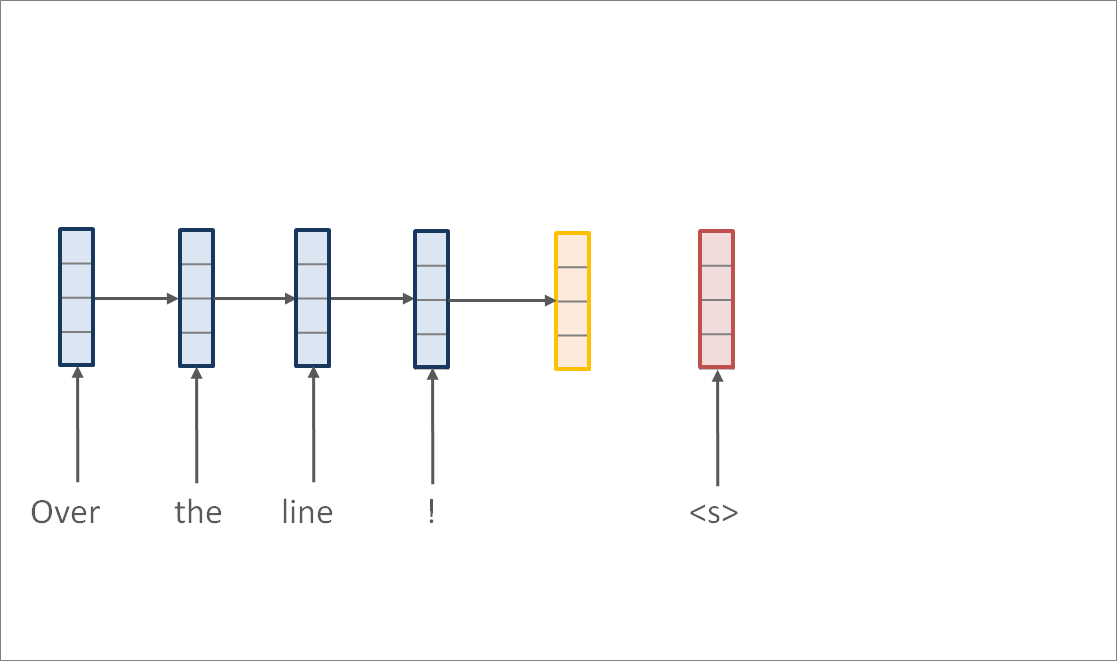
\includegraphics[height=3.5cm, trim={12cm 3cm 7cm 0.5cm}, clip]{nmt-noattn-3}
  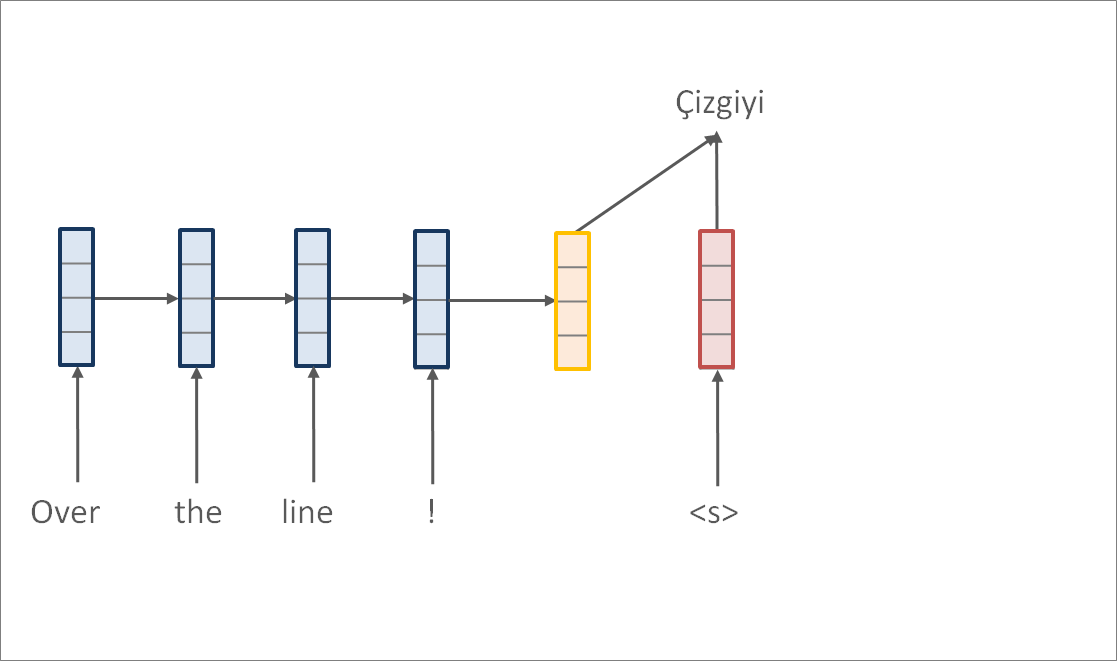
\includegraphics[height=3.5cm, trim={12cm 3cm 7cm 0.5cm}, clip]{nmt-noattn-4}
  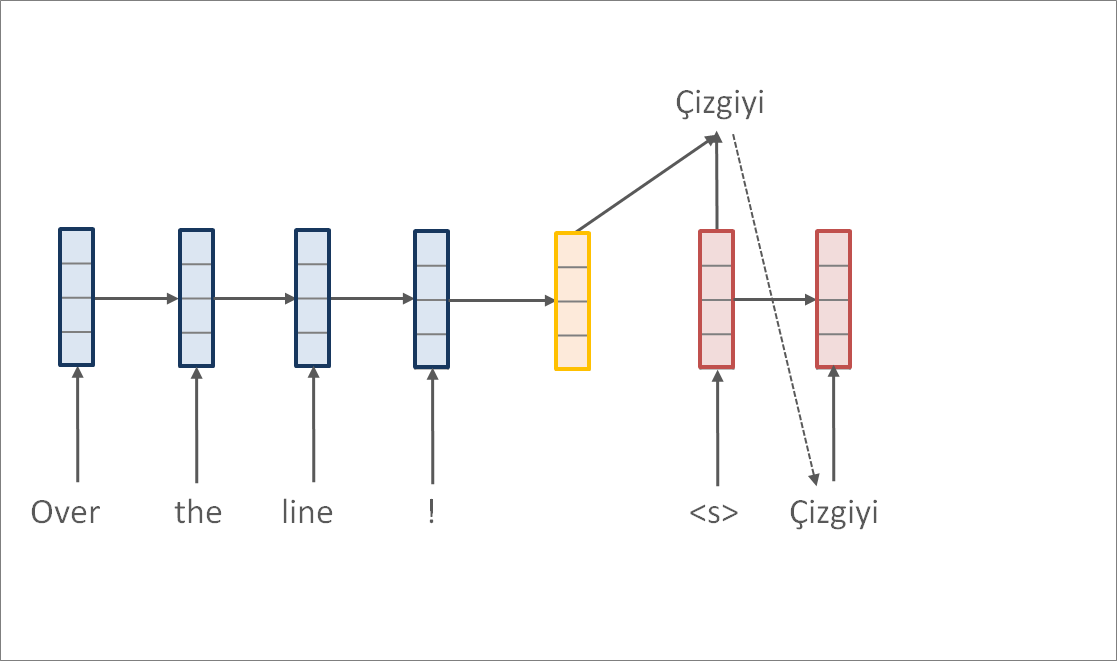
\includegraphics[height=3.5cm, trim={12cm 3cm 0.5cm 0.5cm}, clip]{nmt-noattn-5}
  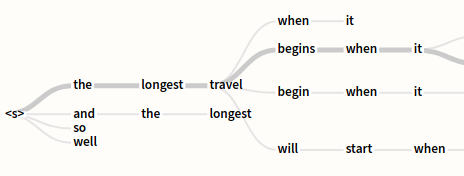
\includegraphics[width=7cm]{beam}


  \end{center}

  \[ y^*_{1:T} = \argmax_{y_{1:T}} f(y_{1:t}; \theta) = \argmax_{y_{1:T}} \sum_{t} \log p(y_{t} | y_{1:t-1}, \cvec; \theta) \] 
  % \pause
  % % \begin{itemize}
  % % \item Note: Completely intractable $O(\text{\#vocab} ^T)$ 
  % % \end{itemize}
\end{frame}

\begin{frame}[fragile]{Heuristic:  Beam Search}
    \begin{center}
  \begin{tikzpicture}[transform canvas = {scale=0.8}]
    \tikzstyle{beam}=[draw, minimum height=0.6cm, anchor=base, text height=5, text depth=0, minimum width=1.5cm,thin, rounded corners, line width=0.03cm]
   \tikzstyle{mat}=[draw=white]
    \tikzset{>=stealth',every on chain/.append style={join},
      every join/.style={->}}

     
       \begin{scope}
   \matrix (G) [matrix of nodes, nodes={beam},inner sep=1mm,row sep=0.03cm, column sep=0.8cm ] {
    \node<1->(G-1-1){a}; & \node<2->(G-1-2){red}; & \node<3->(G-1-3){dog}; & \node<4->(G-1-4){smells}; & \node<5->(G-1-5){home};  & \node<6->(G-1-6){today}; \\
    \node<1->(G-2-1){the}; & \node<2->(G-2-2){dog}; & \node<3->(G-2-3){dog}; & \node<4->(G-2-4){barks}; & \node<5->(G-2-5){quickly}; & \node<6->(G-2-6){Friday}; \\
    \node<1->(G-3-1){red}; & \node<2->(G-3-2){blue}; & \node<3->(G-3-3){cat}; &  \node<4->(G-3-4){barks}; & \node<5->(G-3-5){straight}; & \node<6->(G-3-6){now}; \\    };

    \only<2->{
      \draw[->] (G-1-1.east) -> (G-1-2.west); 
      \draw[->] (G-2-1.east) -> (G-2-2.west); 
      \draw[->] (G-1-1.east) -> (G-3-2.west); 
      \draw[double, line width=0.03cm] (G-3-1.south west) -- (G-3-2.south east);
    }
  
    \only<3->{
      \draw[->] (G-1-2.east) -> (G-2-3.west); 
      \draw[->] (G-3-2.east) -> (G-3-3.west); 
      \draw[->] (G-3-2.east) -> (G-1-3.west); 
      \draw[double, line width=0.03cm] (G-3-1.south west) -- (G-3-3.south east);
    }
    
 \only<4->{
    \draw[->] (G-1-3.east) -> (G-3-4.west); 
    \draw[->] (G-2-3.east) -> (G-2-4.west); 
    \draw[->] (G-1-3.east) -> (G-1-4.west); 
    \draw[double, line width=0.03cm] (G-3-1.south west) -- (G-3-4.south east);
}
 \only<6->{
    \draw[->] (G-1-5.east) -> (G-1-6.west); 
    \draw[->] (G-1-5.east) -> (G-3-6.west); 
    \draw[->] (G-2-5.east) -> (G-2-6.west); 
    \draw[double, line width=0.03cm] (G-3-1.south west) -- (G-3-6.south east);
}

 \only<5->{
    \draw[->] (G-3-4.east) -> (G-1-5.west); 
    \draw[->] (G-3-4.east) -> (G-2-5.west); 
    \draw[->] (G-3-4.east) -> (G-3-5.west); 
    \draw[double, line width=0.03cm] (G-3-1.south west) -- (G-3-5.south east);
}
         \node[left=0.2cm of G]{K};
         \node[below=0.1cm of G]{T};

\end{scope}
\end{tikzpicture}
    \end{center}
   
\air 
    \air



  For time $t$:
   \begin{enumerate}
   \item Compute the score of every possible next word for each sequence,
     \[f(y_t, y_{1:t-1}^{(k)}) \gets \log p(y_{t}\ |\ y^{(k)}_{1:t-1}, \cvec) + \log p(y^{(k)}_{1:t-1} \ |\  \cvec) \]
   \item Prune to only the $K$ highest-scoring target sequences, 
     \[y_{1:t}^{(1:K)} \gets K\argmax_{y_{1:t}} f(y_t, y_{1:t-1}^{(k)})\]  
   \end{enumerate}


  % \begin{enumerate}
  % \item Start with $K$ partial starting hypotheses $\wvec^{(1:K)}$
  % \item For timesteps $t$ from  $1$ to $T$:
  %  \begin{enumerate}
  %  \item Compute for all $k, \wvec_{t}$
  %    \[s(\wvec_t, k) \gets \log p(\wvec_{t} | \wvec^{(k)}_{1:t-1}, \cvec; \theta) + \log p(\wvec^{(k)}_{1:t-1}| \cvec;\theta) \]
  %  \item Save $K$ highest scoring target sequences
  %    \[\wvec_{1:t+1}^{(1:K)} \gets K\arg\max_{\wvec_t, k} s(\wvec_t, k)\]  
  %  \end{enumerate}
  % \end{enumerate}
  \pause
  % \begin{itemize}
  % \item Note: Requires computing $p(\wvec_{t} | \wvec^{(k)}_{1:t-1}, \cvec; \theta)$ for many  $\wvec^{(k)}_{1:t-1}$ 
  % \end{itemize}
\end{frame}

% \begin{frame}[fragile]{Beam Search Example} ($K=3$)

  
%     \begin{center}
%   \begin{tikzpicture}[transform canvas = {scale=0.8}]
%     \tikzstyle{beam}=[draw, minimum height=0.6cm, anchor=base, text height=5, text depth=0, minimum width=1.5cm,thin, rounded corners, line width=0.03cm]
%    \tikzstyle{mat}=[draw=white]
%     \tikzset{>=stealth',every on chain/.append style={join},
%       every join/.style={->}}

     
%        \begin{scope}
         
%    \matrix (G) [matrix of nodes, nodes={beam},inner sep=1mm,row sep=0.03cm, column sep=0.8cm ] {
%     \node<1->(G-1-1){a}; & \node<2->(G-1-2){red}; & \node<3->(G-1-3){dog}; & \node<4->(G-1-4){smells}; & \node<5->(G-1-5){home};  & \node<6->(G-1-6){today}; \\
%     \node<1->(G-2-1){the}; & \node<2->(G-2-2){dog}; & \node<3->(G-2-3){dog}; & \node<4->(G-2-4){barks}; & \node<5->(G-2-5){quickly}; & \node<6->(G-2-6){Friday}; \\
%     \node<1->(G-3-1){red}; & \node<2->(G-3-2){blue}; & \node<3->(G-3-3){cat}; &  \node<4->(G-3-4){runs}; & \node<5->(G-3-5){straight}; & \node<6->(G-3-6){now}; \\    };

%     \only<2->{
%       \draw[->] (G-1-1.east) -> (G-1-2.west); 
%       \draw[->] (G-2-1.east) -> (G-2-2.west); 
%       \draw[->] (G-1-1.east) -> (G-3-2.west); 
%       \draw[double, line width=0.03cm] (G-3-1.south west) -- (G-3-2.south east);
%     }
  
%     \only<3->{
%       \draw[->] (G-1-2.east) -> (G-2-3.west); 
%       \draw[->] (G-3-2.east) -> (G-3-3.west); 
%       \draw[->] (G-3-2.east) -> (G-1-3.west); 
%       \draw[double, line width=0.03cm] (G-3-1.south west) -- (G-3-3.south east);
%     }
    
%  \only<4->{
%     \draw[->] (G-1-3.east) -> (G-3-4.west); 
%     \draw[->] (G-2-3.east) -> (G-2-4.west); 
%     \draw[->] (G-1-3.east) -> (G-1-4.west); 
%     \draw[double, line width=0.03cm] (G-3-1.south west) -- (G-3-4.south east);
% }
%  \only<6->{
%     \draw[->] (G-1-5.east) -> (G-1-6.west); 
%     \draw[->] (G-1-5.east) -> (G-3-6.west); 
%     \draw[->] (G-2-5.east) -> (G-2-6.west); 
%     \draw[double, line width=0.03cm] (G-3-1.south west) -- (G-3-6.south east);
% }

%  \only<5->{
%     \draw[->] (G-3-4.east) -> (G-1-5.west); 
%     \draw[->] (G-3-4.east) -> (G-2-5.west); 
%     \draw[->] (G-3-4.east) -> (G-3-5.west); 
%     \draw[double, line width=0.03cm] (G-3-1.south west) -- (G-3-5.south east);
% }

% \end{scope}
% \end{tikzpicture}
%     \end{center}
%     \air

% For timesteps $t$ from  $1$ to $T$:
%    \begin{enumerate}
%    \item Compute for all $k, \wvec_{t}$
%      \[f(\wvec_t, \wvec_{1:t-1}^{(k)}) \gets \log p(\wvec_{t} | \wvec^{(k)}_{1:t-1}, \cvec) + \log p(\wvec^{(k)}_{1:t-1}| \cvec) \]
%    \item Replace the $K$ highest scoring target sequences
%      \[\wvec_{1:t}^{(1:K)} \gets K\argmax_{\wvec_{1:t}} (\wvec_t, \wvec_{1:t-1}^{(k)})\]  
%    \end{enumerate}

% \end{frame}


\begin{frame}{Theoretical Issues }
  \begin{enumerate}
  \item Exposure Bias
    \begin{itemize}
    \item Training by conditioning on true $y_{1:t-1}$.
    \end{itemize}
    \air
  \item Metric Bias 
    \begin{itemize}
    \item Training with local NLL, evaluate with hamming-style losses.
    \end{itemize}

    \air
  \item Label Bias  %\cite{Lafferty2001}
    \begin{itemize}
    \item Locally normalized models have known pathological issues.
    \end{itemize}

  \end{enumerate}
\end{frame}

\begin{frame}{Work}
  Can we exploit the nature of discrete sequences to improve 
  deep learning models for text generation and translation? 

  \begin{center}
  \begin{tikzpicture}

    % \node at (10mm, 15mm) {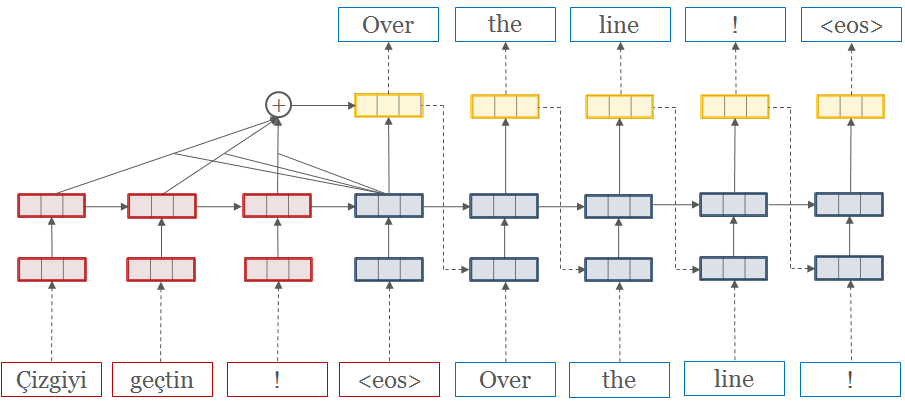
\includegraphics[width=2cm]{nmt}};


    \node[rounded corners, draw] (ana) at (-15mm, 15mm) {Analysis};


    \node[rounded corners, fill=yellow,  draw] (meth) at (0mm, 30mm) {\ Methods\phantom{p}};

    \node[rounded corners, draw] (app) at (25mm, 30mm) {Applications};


    \node[rounded corners, draw] (und) at (35mm, 15mm) {Understanding};


    \node[rounded corners, fill=yellow,  draw] (dep) at (25mm, 0mm){Deployment};

    \node[rounded corners, fill=yellow, draw] (imp) at (0, 0) {Implement};


    \draw (ana) -- (meth) --(app) -- (und) -- (dep) -- (imp) -- (ana);

  \end{tikzpicture}
  \end{center}


\end{frame}

% \begin{frame}{\structure{Related Work:} Modify training data}
%   \air 
%   \begin{itemize}
%   \item Data as Demonstrator \Cite{Venkatraman}, Scheduled Sampling \Cite{Bengio2015}
%   \end{itemize}
%   \air 

%   \centerline{\structure{Related Work:} Use Reinforcement Learning}
%   \air 
%   \begin{itemize}
%   \item MIXER \Cite{Ranzato2016}
%   \item Actor-Critic \Cite{Bahdanau2016}
%   \end{itemize}
  
%   \pause

%   Opinion: 
%   \begin{itemize}
%   \item 
%     DAD methods only address exposure bias, 
%   \item RL is too strong a hammer .
%   \end{itemize}

%   % \begin{itemize}
%   % \item 
%   % \end{itemize}
% \end{frame}


\begin{frame}{Seq2Seq as Beam Search Optimization}

  Main Idea: Replace next word model with a sequence model $f$. 

  
  \air 

  Applications:

  \begin{itemize}
  \item (1) Sequence-to-Sequence as Beam Search Optimization 
    \air 
  \item (2) Sequence Knowledge Distillation.
    \air 
  \end{itemize}
\end{frame}

\begin{frame}{Scoring a Sequence $f$}
  \begin{center}
    % \structure{(Idea 1)} Replace local softmax with sequence scorer 
    % \air 
    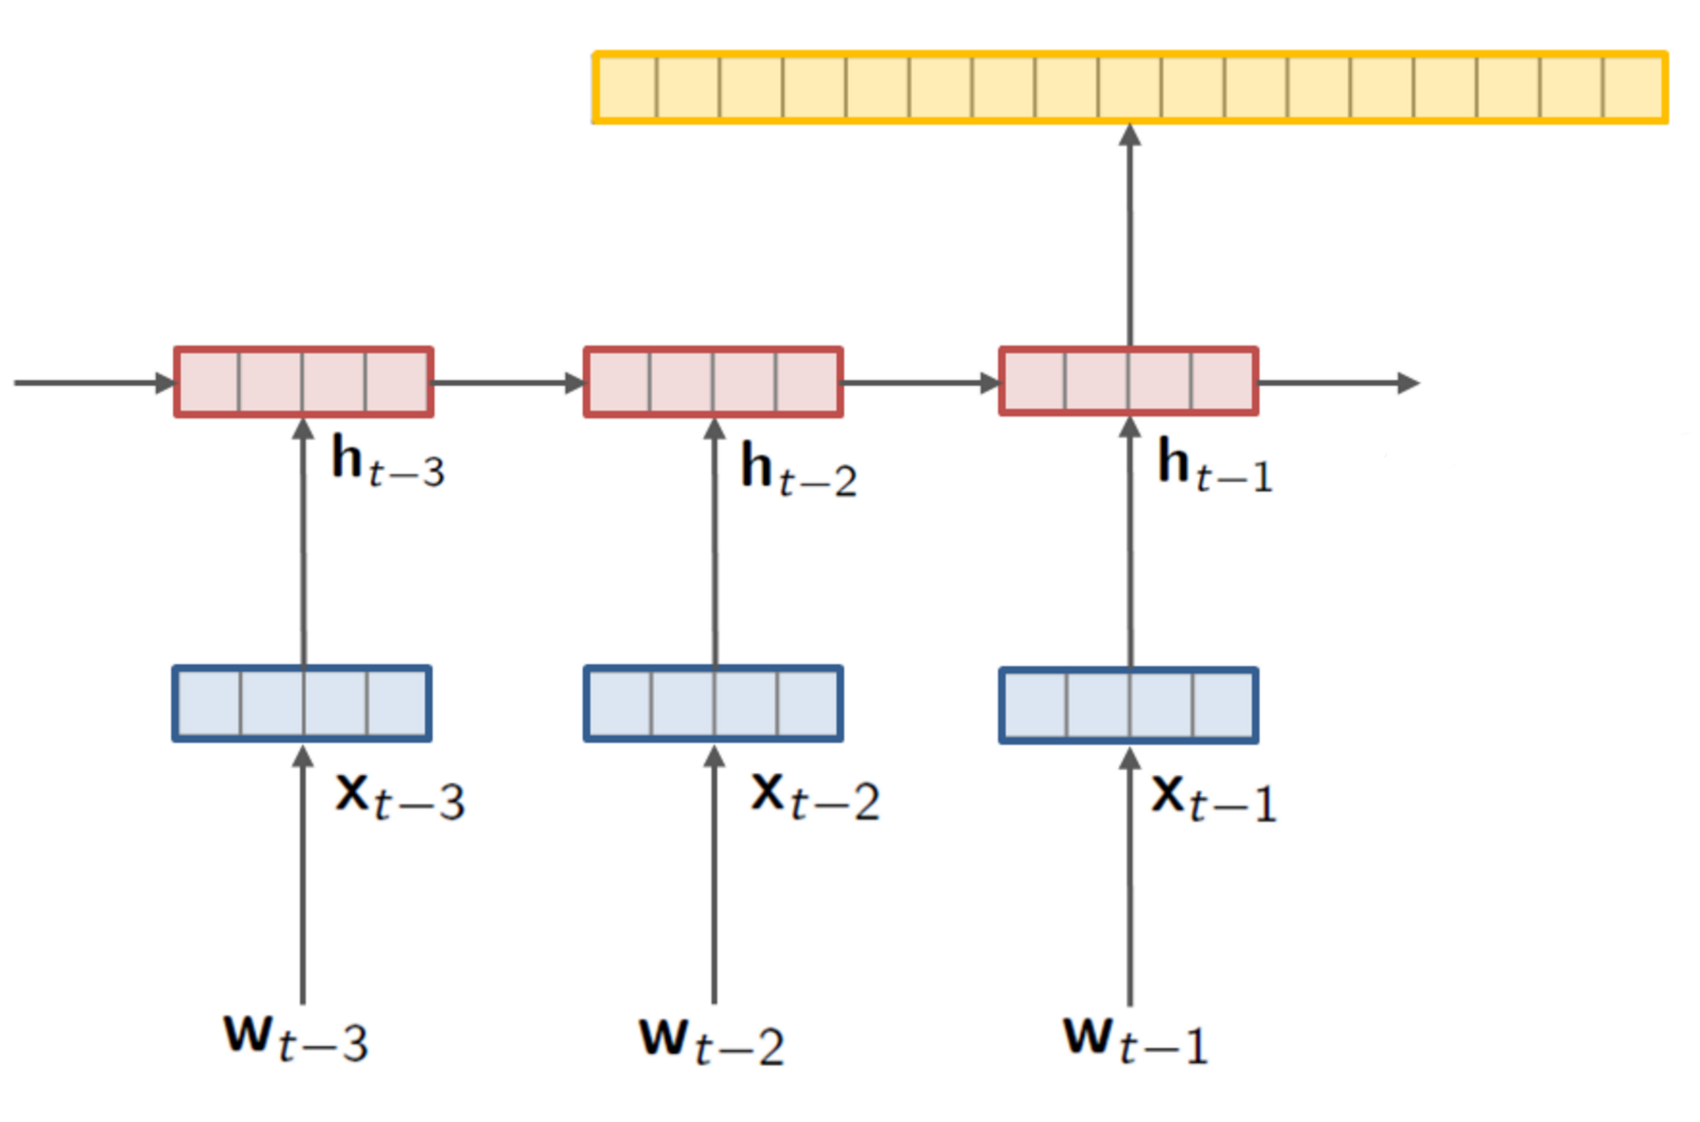
\includegraphics[width=0.6\textwidth]{rnnlm6}
  \end{center}

  Same model, but replace 
  $  \log p(\wvec_{t} | \wvec^{(k)}_{1:t-1}, \cvec; \theta)$
  with unnormalized 
  $f(\wvec_t, \wvec_{1:t-1}^{(k)}, \cvec; \theta)$
\end{frame}

\begin{frame}{(Idea 2)} Run beam search during training
  \begin{enumerate}
  \item Start with $K$ partial starting hypotheses $\wvec^{(1:K)}$
  \item For timesteps $t$ from  $1$ to $T$:
   \begin{enumerate}
   \item Compute for all $k, \wvec_{t}$
     \only<1>{
     \[s(\wvec_t, \wvec_{1:t-1}^{(k)}) \gets \alert{\log p(\wvec_{t} | \wvec^{(k)}_{1:t-1}, \cvec; \theta) + \log p(\wvec^{(k)}_{1:t-1}| \cvec;\theta)} \]
   }
   \only<2>{
     \[s(\wvec_t, \wvec_{1:t-1}^{(k)})  \gets  \structure{f(\wvec_t, \wvec_{1:t-1}^{(k)}, \cvec; \theta)} \]
   }
   \item Replace the  $K$ highest scoring target sequences
     \[\wvec_{1:t}^{(1:K)} \gets K\argmax_{\wvec_{1:t}} s(\wvec_t, \wvec_{1:t-1}^{(k)})\]  
   \end{enumerate}
  \end{enumerate}

\end{frame}


\begin{frame}{\structure{(Idea 3)} Replace local training objective with beam-search margin}

  New Objective: 
  \begin{itemize}

  \item Margin between target seq $y$ and last seq on beam $\wvec^{(K)}$  
  \end{itemize}
\begin{align*}
 \mathcal{L}&(\theta) = \sum_{t} \Delta(y_{1:t}, \wvec_{1:t}^{K}) \left[1 - f(y_t, y_{1:t-1}, \cvec) +  f(\wvec_t^{(K)}, \wvec_{1:t-1}^{(K)}, \cvec) \right] 
\end{align*}

\begin{itemize}
  \item Slack-rescaled, margin-based sequence criterion, at each time step.  
\item When violation occurs, target replaces current beam (learning as search optimization \cite{daume05learning})
\end{itemize}

\end{frame}

\begin{frame}[fragile]{ Beam Search Optimization Example ($K=3$)}
  \begin{center}
    \begin{center}
     
    \end{center}
    \air
    \air
    \air
    \air

  \begin{tikzpicture}[transform canvas = {scale=0.8}]
  \tikzstyle{beam}=[draw, minimum height=0.6cm, anchor=base, text height=5, text depth=0, minimum width=1.5cm,thin, rounded corners, line width=0.03cm]
  \tikzstyle{mat}=[draw=white]
\tikzset{>=stealth',every on chain/.append style={join},
         every join/.style={->}}

     
       % \node[draw = white, yshift=1.8cm]{Time Step};
       %\node[draw = white, xshift=-7.5cm, yshift=0.5cm]{Beam:};
       \begin{scope}
         

   \matrix (G) [matrix of nodes, nodes={beam},inner sep=1mm,row sep=0.03cm, column sep=0.8cm ] {
    \node<1->[fill=yellow](G-1-1){\textcolor{blue}{a}}; & \node<2->[fill=yellow](G-1-2){red}; & \node<3->[fill=lightgray](G-1-3){\textcolor{blue}{dog}}; & \node<4->(G-1-4){smells}; & \node<5->[fill=lightgray](G-1-5){\textcolor{red}{home}};  & \node<6->[fill=lightgray](G-1-6){\textcolor{red}{today}}; \\
    \node<1->(G-2-1){the}; & \node<2->(G-2-2){dog}; & \node<3->[fill=yellow](G-2-3){dog}; & \node<4->(G-2-4){barks}; & \node<5->[fill=yellow](G-2-5){quickly}; & \node<6->(G-2-6){Friday}; \\
    \node<1->(G-3-1){red}; & \node<2->[fill=lightgray](G-3-2){\textcolor{blue}{blue}}; & \node<3->(G-3-3){cat}; &  \node<4->[fill=lightgray](G-3-4){\textcolor{blue}{barks}}; & \node<5->(G-3-5){straight}; & \node<6->[](G-3-6){now}; \\
    & & & \node<4->[fill=yellow](G-4-4){runs}; & & \node<6->[fill=yellow](G-4-6){today}; \\
    };

    \only<2->{
      \draw[->] (G-1-1.east) -> (G-1-2.west); 
      \draw[->] (G-2-1.east) -> (G-2-2.west); 
      \draw[->] (G-1-1.east) -> (G-3-2.west); 
      \draw[double, line width=0.03cm] (G-3-1.south west) -- (G-3-2.south east);
    }
  
    \only<3->{
      \draw[->] (G-1-2.east) -> (G-2-3.west); 
      \draw[->] (G-3-2.east) -> (G-3-3.west); 
      \draw[->] (G-3-2.east) -> (G-1-3.west); 
      \draw[double, line width=0.03cm] (G-3-1.south west) -- (G-3-3.south east);
    }
    
 \only<4->{
    \draw[->] (G-2-3.east) -> (G-4-4.west); 
    \draw[->] (G-1-3.east) -> (G-3-4.west); 
    \draw[->] (G-2-3.east) -> (G-2-4.west); 
    \draw[->] (G-1-3.east) -> (G-1-4.west); 
    \draw[double, line width=0.03cm] (G-3-1.south west) -- (G-3-4.south east);
}
 \only<6->{
    \draw[->] (G-1-5.east) -> (G-1-6.west); 
    \draw[->] (G-1-5.east) -> (G-3-6.west); 
    \draw[->] (G-2-5.east) -> (G-2-6.west); 
    \draw[->] (G-2-5.east) -> (G-4-6.west); 
    \draw[double, line width=0.03cm] (G-3-1.south west) -- (G-3-6.south east);
}

    % \draw[->] (G-3-2.east) -> (G-3-3.west); 
    % \draw[->] (G-3-2.east) -> (G-1-3.west); 

 \only<5->{
    \draw[->, dashed] (G-4-4.east) -> (G-1-5.west); 
    \draw[->, dashed] (G-4-4.east) -> (G-2-5.west); 
    \draw[->, dashed] (G-4-4.east) -> (G-3-5.west); 
    \draw[double, line width=0.03cm] (G-3-1.south west) -- (G-3-5.south east);
}

       \end{scope}
    % \draw(G-1-1.north east) rectangle (G-3-1.south west);
    % \draw(G-1-2.north east) rectangle (G-3-2.south west);

    % \begin{scope}[yshift=-2.8cm]

    %   \matrix (G) [matrix of nodes,nodes={beam}, inner sep=1mm,row sep=0.06cm,column sep=0.8cm ] {
    %     \node[fill=yellow](G-1-1){a}; & \node[fill=yellow](G-1-2){red}; & \node[fill=yellow](G-1-3){dog}; & \node[fill=yellow](G-1-4){runs}; & \node[fill=yellow](G-1-5){quickly}; & \node[fill=yellow](G-1-6){today}; \\
    %      & \node[fill=lightgray](G-2-2){\textcolor{blue}{blue}}; & \node[fill=lightgray](G-2-3){\textcolor{blue}{dog}}; & \node[fill=lightgray](G-2-4){\textcolor{blue}{barks}}; & \node[fill=lightgray](G-2-5){\textcolor{red}{home}}; & \node[fill=lightgray](G-2-6){\textcolor{red}{today}}; \\
    %   };
    % \draw[->] (G-1-1.east) -> (G-1-2.west); 
    % \draw[->] (G-1-2.east) -> (G-1-3.west); 
    % \draw[->] (G-1-3.east) -> (G-1-4.west); 
    % \draw[->] (G-1-4.east) -> (G-1-5.west); 
    % \draw[->] (G-1-5.east) -> (G-1-6.west); 

    % \draw[->] (G-1-1.east) -> (G-2-2.west); 
    % \draw[->] (G-2-2.east) -> (G-2-3.west); 
    % \draw[->] (G-2-3.east) -> (G-2-4.west); 
    % \draw[->] (G-1-4.east) -> (G-2-5.west); 
    % \draw[->] (G-2-5.east) -> (G-2-6.west); 
      
    % \end{scope}
\end{tikzpicture}
  \end{center}  

  \air 
  \air 
% \begin{align*}
%  \mathcal{L}&(\theta) = \sum_{t} \Delta(\wvec_{1:t}, \wvec_{1:t}^{(K)}) \left[1 - f(\wvec_t, \wvec_{1:t-1}, \cvec) +  f(\wvec_t^{(K)}, \wvec_{1:t-1}^{(K)}, \cvec) \right] 
% \end{align*}

  \begin{itemize}
  \item Color \textcolor{yellow}{Gold}: target sequence $y$
  \item Color \textcolor{gray}{Gray}: violating sequence $\wvec^{(K)}$
  \end{itemize}
\end{frame}

\begin{frame}[fragile]{Structured Backpropagation}
  \begin{center}
    
  \air 
  \air 

  \begin{tikzpicture}[transform canvas = {scale=0.8}]
    \tikzstyle{beam}=[draw, minimum height=0.6cm, anchor=base, text height=5, text depth=0, minimum width=1.5cm,thin, rounded corners, line width=0.03cm]
    \tikzstyle{mat}=[draw=white]
    \tikzset{>=stealth',every on chain/.append style={join},
      every join/.style={->}}
    
     
       % \node[draw = white, yshift=1.8cm]{Time Step};
       %\node[draw = white, xshift=-7.5cm, yshift=0.5cm]{Beam:};
       \begin{scope}
         

   \matrix (G) [matrix of nodes, nodes={beam},inner sep=1mm,row sep=0.03cm, column sep=0.8cm ] {
     \node[fill=yellow](G-1-1){\textcolor{blue}{a}}; & \node[fill=yellow](G-1-2){red}; & \node[fill=lightgray](G-1-3){\textcolor{blue}{dog}}; & \node(G-1-4){smells}; & \node[fill=lightgray](G-1-5){\textcolor{red}{home}};  & \node[fill=lightgray](G-1-6){\textcolor{red}{today}}; \\
     \node(G-2-1){the}; & \node(G-2-2){dog}; & \node[fill=yellow](G-2-3){dog}; & \node(G-2-4){barks}; & \node[fill=yellow](G-2-5){quickly}; & \node(G-2-6){Friday}; \\
     \node(G-3-1){red}; & \node[fill=lightgray](G-3-2){\textcolor{blue}{blue}}; & \node(G-3-3){cat}; &  \node[fill=lightgray](G-3-4){\textcolor{blue}{barks}}; & \node(G-3-5){straight}; & \node[](G-3-6){now}; \\
     & & & \node[fill=yellow](G-4-4){runs}; & & \node[fill=yellow](G-4-6){today}; \\
    };


    \draw[->] (G-1-1.east) -> (G-1-2.west); 
    \draw[->] (G-2-1.east) -> (G-2-2.west); 
    \draw[->] (G-1-1.east) -> (G-3-2.west); 
    \draw[double, line width=0.03cm] (G-3-1.south west) -- (G-3-2.south east);


    \draw[->] (G-1-2.east) -> (G-2-3.west); 
    \draw[->] (G-3-2.east) -> (G-3-3.west); 
    \draw[->] (G-3-2.east) -> (G-1-3.west); 
    \draw[double, line width=0.03cm] (G-3-1.south west) -- (G-3-3.south east);

    \draw[->] (G-2-3.east) -> (G-4-4.west); 
    \draw[->] (G-1-3.east) -> (G-3-4.west); 
    \draw[->] (G-2-3.east) -> (G-2-4.west); 
    \draw[->] (G-1-3.east) -> (G-1-4.west); 
    \draw[double, line width=0.03cm] (G-3-1.south west) -- (G-3-4.south east);

    \draw[->] (G-1-5.east) -> (G-1-6.west); 
    \draw[->] (G-1-5.east) -> (G-3-6.west); 
    \draw[->] (G-2-5.east) -> (G-2-6.west); 
    \draw[->] (G-2-5.east) -> (G-4-6.west); 
    \draw[double, line width=0.03cm] (G-3-1.south west) -- (G-3-6.south east);


    % \draw[->] (G-3-2.east) -> (G-3-3.west); 
    % \draw[->] (G-3-2.east) -> (G-1-3.west); 


    \draw[->, dashed] (G-4-4.east) -> (G-1-5.west); 
    \draw[->, dashed] (G-4-4.east) -> (G-2-5.west); 
    \draw[->, dashed] (G-4-4.east) -> (G-3-5.west); 
    \draw[double, line width=0.03cm] (G-3-1.south west) -- (G-3-5.south east);


       \end{scope}

       \begin{scope}[yshift=-2.8cm]

      \matrix (G) [matrix of nodes,nodes={beam}, inner sep=1mm,row sep=0.06cm,column sep=0.8cm ] {
        \node[fill=yellow](G-1-1){a}; & \node[fill=yellow](G-1-2){red}; & \node[fill=yellow](G-1-3){dog}; & \node[fill=yellow](G-1-4){runs}; & \node[fill=yellow](G-1-5){quickly}; & \node[fill=yellow](G-1-6){today}; \\
         & \node[fill=lightgray](G-2-2){\textcolor{blue}{blue}}; & \node[fill=lightgray](G-2-3){\textcolor{blue}{dog}}; & \node[fill=lightgray](G-2-4){\textcolor{blue}{barks}}; & \node[fill=lightgray](G-2-5){\textcolor{red}{home}}; & \node[fill=lightgray](G-2-6){\textcolor{red}{today}}; \\
      };
    \draw[->] (G-1-1.east) -> (G-1-2.west); 
    \draw[->] (G-1-2.east) -> (G-1-3.west); 
    \draw[->] (G-1-3.east) -> (G-1-4.west); 
    \draw[->] (G-1-4.east) -> (G-1-5.west); 
    \draw[->] (G-1-5.east) -> (G-1-6.west); 

    \draw[->] (G-1-1.east) -> (G-2-2.west); 
    \draw[->] (G-2-2.east) -> (G-2-3.west); 
    \draw[->] (G-2-3.east) -> (G-2-4.west); 
    \draw[->] (G-1-4.east) -> (G-2-5.west); 
    \draw[->] (G-2-5.east) -> (G-2-6.west); 
      
    \end{scope}
  \end{tikzpicture}  
  \end{center}
  \vspace{2cm}
  \vspace{1cm}
  
  \begin{itemize}
  \item Margin gradients are sparse, only violating sequences get updates.
  \item Backprop as efficient as standard models.
  \end{itemize}
\end{frame}

% \begin{frame}
%   \begin{center}
%     \structure{(Idea 3)} Extension: Incorporate hard constraints at training.
%   \end{center}

% \end{frame}

\begin{frame}{Theoretical Issues Revisited}
  \begin{itemize}

  \item Exposure Bias
    \begin{itemize}
    \item Beam search at training
    \end{itemize}
    \air
  \item Train/Test Loss Mismatch 
    \begin{itemize}
    \item Slack-rescaled margin can capture correct loss.
    \end{itemize}

    \air
  \item Label Bias  \cite{Lafferty2001}
    \begin{itemize}
    \item Sequence regression is not locally normalized
    \end{itemize}

  \end{itemize}
\end{frame}


\begin{frame}{Experiments}
  \air 

  Experiments run on three different seq2seq baseline tasks

  \begin{itemize}
  \item Word Ordering
    \air
  \item Dependency Parsing
    \air 
  \item Machine Translation
  \end{itemize}



  Details:
  \begin{itemize}
  \item Utilize our \textit{seq2seq-attn} code, very strong attention-based system 
  \item Pretrained with NLL. 
  \item Trained with a curriculum to gradually increase beam size.
  \end{itemize}
 
\end{frame}


\begin{frame}{Results}
  \vspace{-0.2cm}
  \begin{table}
  \centering
    \small
  \begin{tabular}{lccc}
    \toprule
    & $K_e$ = 1 & $K_e$ = 5 & $K_e$ = 10 \\ 
    \midrule
     & \multicolumn{3}{c}{Word Ordering (BLEU) } \\ 
    \midrule
    seq2seq & 25.2 & 29.8 & 31.0 \\
    BSO     & 28.0 & 33.2 & 34.3 \\
    BSO-Con & \textbf{28.6} & \textbf{34.3} & \textbf{34.5} \\
    \midrule
%   \end{tabular}
%   \label{tab:wo}
% \end{table}


% \begin{table}
%   \centering
%   \hspace*{-0.3cm}\begin{tabular}{lccc}
%     \toprule
    & \multicolumn{3}{c}{Dependency Parsing (UAS/LAS) } \\ 
    % \midrule
    seq2seq & \textbf{87.33/82.26} & 88.53/84.16 & 88.66/84.33\\
    BSO & 86.91/82.11 & 91.00/\textbf{87.18} & 91.17/\textbf{87.41} \\
    BSO-Con & 85.11/79.32 & \textbf{91.25}/86.92 & \textbf{91.57}/87.26 \\
    % \midrule
    % Andor & 93.17/91.18 & - & - \\ 
    % \bottomrule

    \midrule
    & \multicolumn{3}{c}{Machine Translation (BLEU) } \\ 
    % &  $K_e$ = 1 & $K_e$ = 5 & $K_e$ = 10 \\ 
    % \midrule
    seq2seq & 22.53 & 24.03 & 23.87 \\
    BSO, SB-$\Delta$, $K_t$=6 & \textbf{23.83} & \textbf{26.36} & \textbf{25.48} \\
    % \midrule
    XENT & 17.74 & $\leq$ 20.5 & $\leq$ 20.5 \\
    DAD & 20.12 & $\leq$ 22.5 & $\leq$ 23.0 \\ 
    MIXER & 20.73 & - & $\leq$ 22.0 \\    
    \bottomrule
  \end{tabular}
  \label{tab:mtfinal}
\end{table}

\end{frame}


% \begin{frame}

% \end{frame}

\begin{frame}
  \centerline{\structure{Related Work: Compressing Deep Models}}
\air

\begin{itemize}
\item \textbf{Pruning}: Prune weights based on importance criterion 
\cite{LeCun1990,Han2016}
\item \textbf{Knowledge Distillation}: Train a \textit{student} model to learn 
from a \textit{teacher} model \cite{Bucila2006,Ba2014,Hinton2015}.
\end{itemize}
\air
Other methods: 
\begin{itemize}
\item low-rank matrix factorization of weight matrices \cite{Denton2014}
\item weight binarization \cite{Lin2016}
\item weight sharing \cite{Chen2015}
\end{itemize}
\end{frame}



% \begin{frame}
% \centerline{\structure{Word-Level Knowledge Distillation}}
% \air 
% \air

% \begin{columns}
% \begin{column}{6.5cm}
% Teacher network: $q(\yvec \given  ; \theta_T$)  \\
% \air
% \air
% Student network: $p(\yvec \given \xvec ; \theta$)
% \end{column}
% \begin{column}{5.5cm}
% 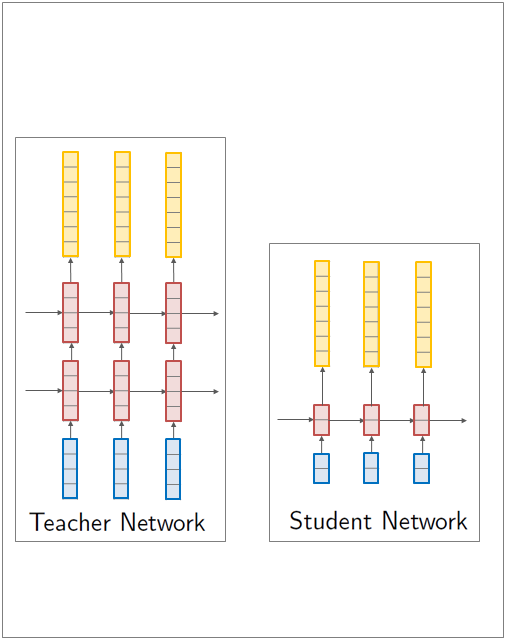
\includegraphics[width=5.5cm]{word-kd-1}
% \end{column}
% \end{columns}
% \end{frame}

\begin{frame}{Baseline Model}
\air 


\begin{columns}
\begin{column}{6.5cm}
Standard model minimize $\text{NLL}(\theta)$: 
\air
$$-\sum_t \log p(\wvec_t=y_t \given \wvec_{1:t-1}, \cvec ; \theta)$$

where $y_t$ is the ground truth word at time $t$.

\air 

Cross-entropy with ground truth.

\end{column}
\begin{column}{5.5cm}
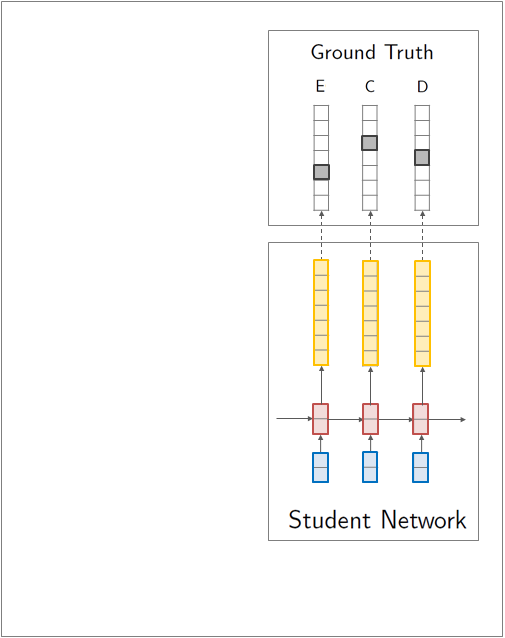
\includegraphics[width=5.5cm]{word-kd-0}
\end{column}
\end{columns}
\end{frame}

% \begin{frame}
% \centerline{\structure{Word-Level Knowledge Distillation}}
% \air
% \air
% \begin{columns}
% \begin{column}{6.5cm}
% Teacher network: $q(\wvec_{t} | \wvec_{1:t-1}, \cvec  ; \theta_T$)  \\
% \air
% \air
% Student network: $p(\wvec_{t} | \wvec_{1:t-1}, \cvec; \theta$)
% \end{column}
% \begin{column}{5.5cm}
% 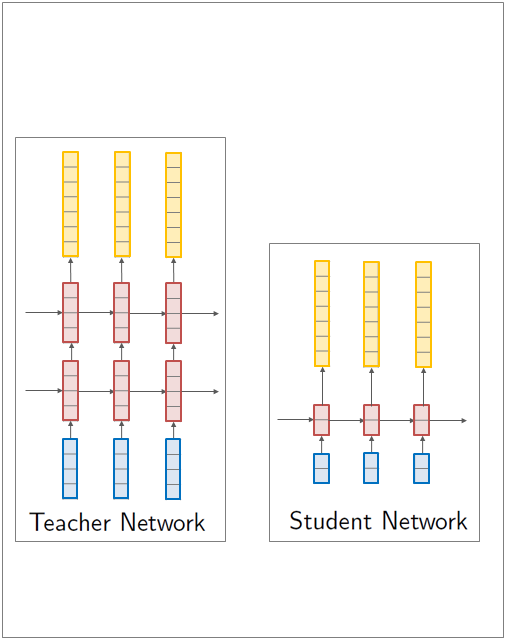
\includegraphics[width=5.5cm]{word-kd-1}
% \end{column}
% \end{columns}
% \end{frame}


\begin{frame}{Word-Level Knowledge Distillation}
\air 
\begin{columns}
\begin{column}{6.5cm}

Teacher network: $q(\wvec_{t} | \wvec_{1:t-1}, \cvec  ; \theta_T$)  
\air 

Minimize cross-entropy between teacher and student distribution  $\mathcal{L}_{\text{WORD-KD}}(\theta)$ \\

\begin{align*}
-\sum_t \sum_v &q(\wvec_t=v \given \wvec_{1: t-1}, \cvec ; \theta_T)\times \\
& \log p(\wvec_t =v \given \wvec_{1: t-1}, \cvec ; \theta)
\end{align*}
\end{column}

\begin{column}{5.5cm}
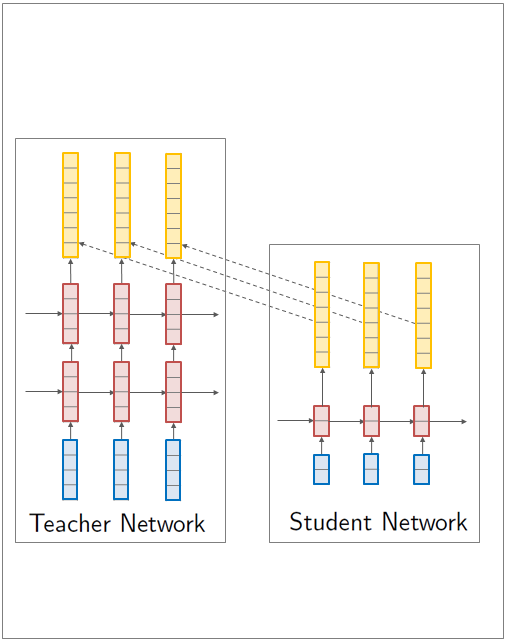
\includegraphics[width=5.5cm]{word-kd-2}
\end{column}
\end{columns}
\end{frame}

% \begin{frame}
% \centerline{\structure{Word-Level Knowledge Distillation}}
% \air
% \begin{columns}
% \begin{column}{6.5cm}
% Add a term for NLL (equivalent to minimizing cross-entropy between student a mixture distribution of teacher/data distributions)  
% \air
% $$\mathcal{L}(\theta) = \alpha\mathcal{L}_{\text{WORD-KD}}(\theta) + (1-\alpha)\mathcal{L}_{\text{NLL}}(\theta)$$
% \air
% $\alpha$ is a hyperparameter (we use $\alpha = 0.5$)
% \end{column}

% \begin{column}{5.5cm}
% 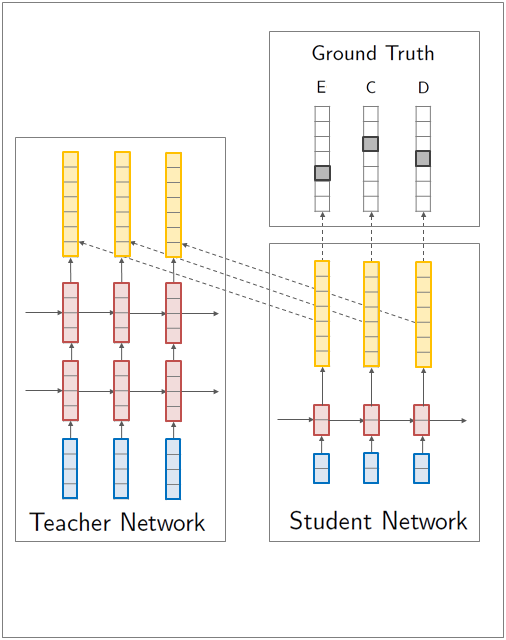
\includegraphics[width=5.5cm]{word-kd-3}
% \end{column}
% \end{columns}
% \end{frame}

\begin{frame}{Sequence-Level Knowledge Distillation}
\air 
\air
\air  

Instead of word NLL, 

\begin{align*}
-\sum_t \sum_v &q(\wvec_t=v \given \wvec_{1: t-1}, \cvec ; \theta_T)\times  \log p(\wvec_t =v \given \wvec_{1: t-1}, \cvec ; \theta)
\end{align*}
 
% $$-\sum_t \log p(\wvec_t=y_t \given \wvec_{1:t-1}, \cvec ; \theta)$$

Minimize cross-entropy between $q$ and $p$ implied \emph{sequence}-distributions 
\[
 -\sum_{\wvec_{1:T}} q(\wvec_{1:T} | \cvec; \theta_T) \times \log p(\wvec_{1:T} | \cvec ; \theta)
\]
\air

Note: Exponential sum over possible $\wvec_{1:T}$ . \\ 
\air
\air

\end{frame}

\begin{frame}{A Simple Approximation}
\air 
\air

%\centerline{Sequence-Level Knowledge Distillation}
\begin{columns}
\begin{column}{6cm}
Approximate $q(\wvec_{1:T} \given \cvec )$ with mode
$$q(\wvec_{1:T} \given \cvec ) \approx \mathbf{1}\{\argmax_{\wvec} q(\wvec_{1:T} \given \cvec )\}$$
\air
Roughly obtained wtih  beam search 
$$ \wvec^*_{1:T} \approx  \argmax_{\wvec_{1:T}} q(\wvec_{1:T} \given \cvec ) $$
\\
Empirically, point estimate captures 
significant mass

\end{column}
\begin{column}{6cm}
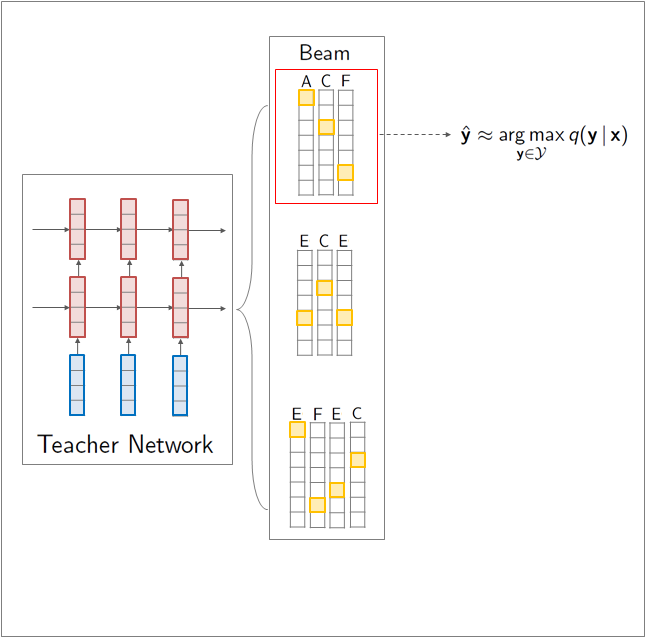
\includegraphics[width=6cm]{seq-kd-1}
\end{column}
\end{columns}
\end{frame}

\begin{frame}{Sequence-Level Knowledge Distillation}

\air  
\begin{columns}
\begin{column}{5.5cm}
\begin{align*}
\mathcal{L}_\text{SEQ-KD}(\theta) &= -\log p(\wvec^*_{1:T} \given \cvec ; \theta)  \\
& \displaystyle \approx   -\sum_{\wvec_{1:T}} q(\wvec_{1:T} | \cvec; \theta_T) \log p(\wvec_{1:T} | \cvec ; \theta)
\end{align*}
Simplest model: train the student model on $\wvec^*$ with NLL
\end{column}
\begin{column}{5.5cm}
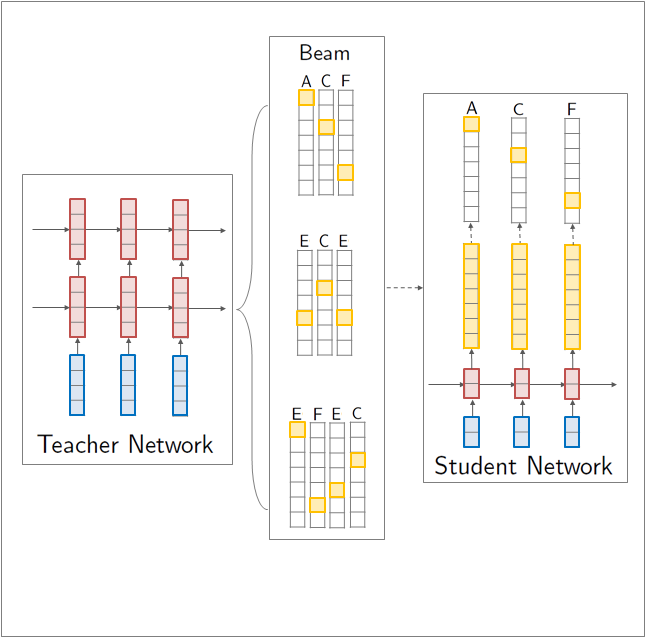
\includegraphics[width=5.5cm]{seq-kd-2}
\end{column}
\end{columns}
\end{frame}

\begin{frame}{Results: English $\rightarrow$ German}
\air
\air
\begin{table}
\centering
\small
\begin{tabular}{lccccrr}
\toprule
Model &    BLEU$_{K=1}$   & $\Delta_{K=1}$ & BLEU$_{K=5}$ & $\Delta_{K=5}$ & PPL & $p(\wvec^*)$ \\
\midrule
$4 \times 1000$ \\
Teacher    & $17.7$ &  $-$ & $19.5$&   $-$ &   $6.7$ &  $1.3\%$ \\
\hspace{1mm} Seq-Inter    & $19.6$ & $+1.9$&  $19.8$& $+0.3$&   $10.4$ & $8.2\%$   \\
\midrule
$2 \times 500$ \\ 
Student  $\,$   & $14.7$ & $-$ & $17.6$&  $-$ &  $8.2$ & $0.9\%$  \\
\hspace{1mm} Word-KD  & $15.4$ & $+0.7$& $17.7$& $+0.1$&  $8.0$ & $1.0\%$  \\
\hspace{1mm} Seq-KD   & $18.9$ & $+\mathbf{4.2}$& $19.0$& $+1.4$&  $22.7$ & $16.9\%$ \\
\hspace{1mm} Seq-Inter  & $18.9$ & $+\mathbf{4.2}$&$19.3$ & $+\mathbf{1.7}$ &  $15.8$ & $7.6\%$  \\
\bottomrule
\end{tabular}

\end{table}
\air
\air
\end{frame}

\begin{frame}{Combining Knowledge Distillation and Pruning}
\air
\air
\begin{table}[t] \label{prune}
\centering
\small
\begin{tabular}{l  r  r c  r }
\toprule
Model & Prune $\%$ & Params & BLEU & Ratio \\
\midrule 
$4 \times 1000$ & $0\%$ &$221$ m& $19.5$& $1 \times$   \\
$2 \times 500$ &  $0\%$& $84$ m& $19.3$& $3 \times$   \\
$2 \times 500$ & $50\%$& $42$ m&  $19.3$ & $5 \times$ \\
$2 \times 500$ &  $80\%$& $17$ m&  $19.1$ & $13 \times$ \\
$2 \times 500$ &  $85\%$& $13$ m&  $18.8$ & $18 \times$ \\
$2 \times 500$ &  $90\%$& $8$ m &  $18.5$  & $26 \times$ \\

\bottomrule
\end{tabular}
\end{table}
\end{frame}


\begin{frame}
  % \centerline{An Application}
  
  \begin{center}
    \includegraphics[height=0.9\textheight]{phonemt}
  \end{center}
\end{frame}

\begin{frame}{Application: }

\end{frame}

